%===============================================================================
%          File: ch1_introduction.tex
%        Author: Juan de Monasterio
%       Created: 08 Feb 2017
%   Description: Chapter 1: Introduction
%===============================================================================

\chapter{Introduction}
\label{cha:intro}


\section{Preamble}

\section{Abstract}\label{section-abstract}


We use mobile phone records for the analysis of mobility patterns and the detection of possible risk zones of Chagas disease in two Latin American countries. We show that geolocalized call records are rich in social and individual information, which can be used to infer whether an individual has lived in an endemic area. We present two case studies, in Argentina and in Mexico, using data provided by mobile phone companies from each country. The risk maps that we generate can be used by health campaign managers to target specific areas and allocate resources more effectively. Finally, we show the value of mobile phone records to predict long-term migrations, which play a crucial role in the spread of Chagas disease.


\section{Introduction}

Chagas disease is a tropical parasitic epidemic of global reach, spread mostly across 21 Latin American countries. The World Health Organization (WHO) estimates more than six million infected people worldwide~\cite{who2016}.  Caused by the \textit{Trypanosoma cruzi} parasite, its transmission occurs mostly in the American endemic regions via the \textit{Triatoma infestans} insect family (also called ``kissing bug", and known by many local names such as ``vinchuca" in Argentina, Bolivia, Chile and Paraguay, and ``chinche" in Central America). In recent years and due to globalization and migrations, the disease has become an %health 
issue in other continents~\cite{schmunis2010chagas}, 
particularly in countries that receive Latin American immigrants such as Spain~\cite{navarro2012chagas} and the United States~\cite{hotez2013unfolding}, 
making it a global health problem.

A crucial characteristic of the infection is that it may last 10 to 30 years in an individual without being detected~\cite{rassi2012american}, which greatly complicates effective detection and treatment. About 30\% of individuals with chronic Chagas disease will develop life-threatening cardiomyopathies or gastrointestinal disorders, whereas 
the remaining individuals will never develop symptoms.
Long-term human mobility (particularly seasonal and permanent rural-urban migration) thus plays a key role in the spread of the epidemic~\cite{briceno2009chagas}. Relevant routes of transmission also include blood transfusion, congenital contagion --with an estimated 14,000 newborns infected each year in the Americas~\cite{OPS2006chagas}--,
organ transplants, 
accidental ingestion of food contaminated by \textit{Trypanosoma cruzi}, and even, in a minor scale, 
by laboratory accidents.
%Aca agregaría las otras vías de transmisión: trasplante de organos, por ingestión accidental de alimentos contaminados con T. cruzi (en italic) y en menor medida por accidentes de laboratorio.
% and worldwide treatment rates of less than 1\%.
% \begin{comment}  en el drive estan las ppt del min salud \end{comment}. 
The spatial dissemination of a congenitally transmitted disease sidesteps the available measures to control risk groups, and shows that individuals who have not been exposed to the disease vector should also be included in detection campaigns.

Mobile phone records contain information about the movements of large subsets of the population of a country, and make them very useful to understand the spreading dynamics of infectious diseases. They have been used to understand the diffusion of malaria in Kenya~\cite{wesolowski2012quantifying} and in Ivory Coast~\cite{enns2013human}, including the refining of infection models~\cite{chunara2013large}. The cited works on Ivory Coast were performed using the D4D (Data for Development) challenge datasets released in 2013. Tizzoni et al.~\cite{tizzoni2014use} compare different mobility models using theoretical approaches, available census data and models based on CDRs interactions to infer movements. They found that the models based on CDRs and mobility census data are highly correlated, illustrating their use as mobility proxies.

Mobile phone data has also been used to predict the geographic spread and timing of Dengue epidemics~\cite{wesolowski2015impact}. This analysis was performed for the country of Pakistan, which is representative of many countries on the verge of countrywide endemic dengue transmission. Other works directly study CDRs to characterize human mobility and other sociodemographic information. A complete survey of mobile traffic analysis articles may be found in~\cite{naboulsi2015mobile}, which also reviews additional studies based on the Ivory Coast dataset mentioned above.


In this work, we discuss the use of mobile phone records --also known as Call Detail Records (CDRs)-- for the analysis of mobility patterns and the detection of possible risk zones of Chagas disease in two Latin American countries. Key health expertise on the subject was provided by the \textit{Mundo Sano} Foundation.
 We generate predictions of population movements between different regions, providing a proxy for the epidemic spread. Our objective is to show that geolocalized call records are rich in social and individual information, which can be used to determine whether an individual has lived in an epidemic area. We present two case studies, in Argentina and in Mexico, using data provided by mobile phone companies from each country. %A discussion of how mobile data was processed is included. 
This is the first work that leverages mobile phone data to better understand the diffusion of the Chagas disease.




%\subsection{Chagas Disease in Argentina and Mexico}

\subsection{Key Facts and Endemic Zone in Argentina}\label{endemic_zone_argentina}

For more than 50 years, vector control campaigns have been underway in Argentina as the main epidemic counter-measure. The \textit{Gran Chaco}, situated in the northern part of the country is home to the disease-carrying triatomines. This region is hyperendemic for the disease~\cite{OPS2014mapa}. A map of this ecoregion is shown in Figure~\ref{fig:granchaco}.

The ecoregion's low socio-demographic conditions further support the parasite's lifecycle, where domestic interactions between humans, triatomines and animals foster the appearance of new infection cases, particularly among rural and poor areas.
% The ecoregion as of today is hyperendemic for the disease.
This region is considered as the endemic zone $E_Z$ in the analysis described in Section~\ref{methods} and Section~\ref{results}.

\begin{figure}[h!]
\centering
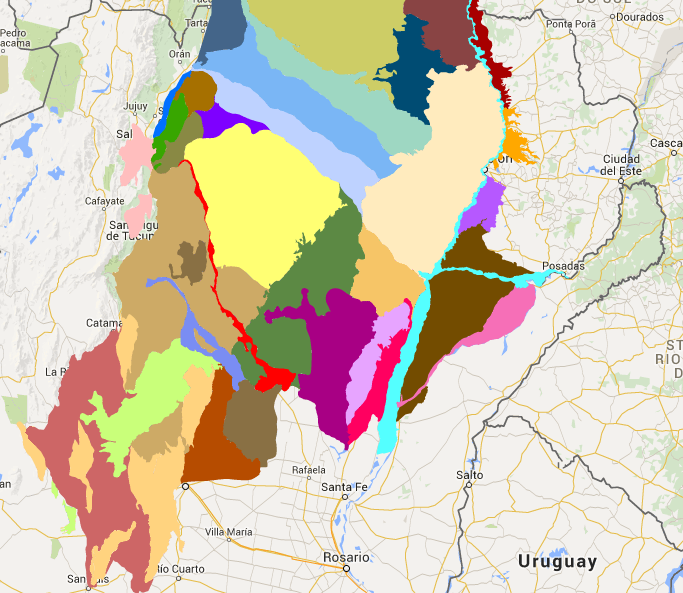
\includegraphics[width=0.75\columnwidth]{figures/Ambientes_GranChaco_TNC-Argentina/Ambientes_GranChaco_TNC-Argentina.png}
\caption{The \textit{Gran Chaco} ecoregion in South America.%
}
% \end{center}
\label{fig:granchaco}
\end{figure}


The dynamic interaction of the triatomine infested areas and the human mobility patterns create a difficult scenario to track down individuals or spots with high prevalence of infected people or transmission risk. Available methods of surveying the state of the Chagas disease in Argentina nowadays are limited to individual screenings of individuals. %The work described here is the first attempt to use mobile phone data to correlate migrations and cellphone usage to understand Chagas epidemic spatial structure. AS: WE ALREADY SAID THIS.

Recent national estimates indicate that there exist between 1.5 and 2 million individuals carrying the parasite, with more than seven million exposed. National health systems face many difficulties to effectively treat the disease. 
In Argentina, less than 1\% of infected people are diagnosed and treated 
(the same statistic holds at the world level).
% (and in Argentina, in particular, less than 1\% of infected people are treated yearly). 
Even though governmental programs have been ongoing for years now~\cite{plan_nacional_chagas}, data on the issue is scarce or hardly accessible. This presents a real obstacle to ongoing research and coordination efforts to tackle the disease in the region.


\subsection{Key Facts and Endemic Zone in Mexico} \label{endemic_zone_mexico}


\begin{figure}[h!]
\centering
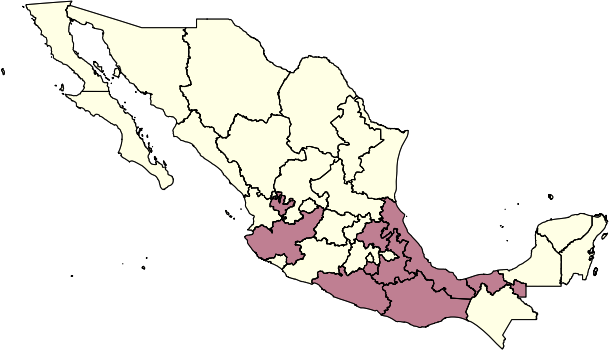
\includegraphics[width=0.75\linewidth]
{figures/Ambientes_Gran_Chaco-Mexico1/Ambientes_Gran_Chaco-Mexico1.png}
\caption{Endemic region $E_Z$ for Mexico.}
\label{fig:endemic_zone_mexico}
\end{figure}

In 2004, the joint work of \textit{Instituto Nacional de Cardiología ``Ignacio Chávez"} and  \textit{Instituto de Biología de la UNAM} resulted in a Chagas disease database for Mexico~\cite{cruz2006chagmex}. Reviewing positive serology in blood banks and human reported cases per state, an epidemic risk map description was produced to geographically situate the disease. Based on this data, we defined the Mexican epidemic area, selecting the states having the top 25\% prevalence rates nationwide. The resulting risk region is shown in Figure~\ref{fig:endemic_zone_mexico}. It covers most of the South region of the country and includes the states of Jalisco, Oaxaca, Veracruz, Guerrero, Morelos, Puebla, Hidalgo and Tabasco.
This region is considered as the endemic zone $E_Z$ for the Mexican case in the analysis described in Sections~\ref{methods}, \ref{results} and \ref{long_term}.



The authors of \cite{carabarin2013chagas} provide an extensive review of the 
research reports on Chagas disease in Mexico.
The review is very critical, stating that there are no effective vector control programs in Mexico;
and that the actual prevalence of the disease 
can only be estimated because no official reporting of cases is performed.
%;
%and in addition, that there is no consensus on the diagnostic methods for 
%Chagas disease in maternity wards and blood banks~\cite{carabarin2013chagas}.

According to \cite{dumonteil1999update}, 
there are a total of 18 endemic areas in Mexico, located in the southeast, and
these areas include the states of Oaxaca, Jalisco, Yucatán, Chiapas, Veracruz,
Puebla, Guerrero, Hidalgo, and Morelos, all of them with rural areas.
Chiapas, Oaxaca, Puebla, Veracruz and Yucatán are among the most affected states (where the prevalence may exceed 10\%), although cases have been reported in most areas of the country
\cite{cruz2006chagmex,dumonteil1999update}.
Despite the lack of official reports, an estimate of the number of \textit{Trypanosoma cruzi} infections by state in the country
indicates that the number of potentially
affected people in Mexico is about 5.5 million~\cite{carabarin2013chagas}.
Mexico, together with Bolivia, Colombia, and Central
America, are among the countries most affected by this 
\textit{neglected tropical disease} (NTD)~\cite{hotez2013innovation}.
The disease doesn't know about borders:
Chagas and other neglected tropical diseases present in the north of Mexico remain highly endemic in the south of Texas as well~\cite{hotez2012texas}.

In recent years there has been a focus on treating the disease with two available
medications, benznidazole or nifurtimox. A study
that explores the access to these two drugs in Mexico 
shows that less than 0.5\% of those who are infected with
the disease received treatment in Mexico in years~\cite{manne2013barriers}.


People from endemic areas of Chagas disease tend to migrate to industrialized cities of the country, mainly Mexico City, in search of jobs. 
In accordance with this movement, a report showed
that infected children under 5 year of age are frequently distributed in urban
rather than in rural areas, indicating that the disease is becoming urbanized in
Mexico~\cite{guzman2001epidemiology}.
Therefore, as in the Argentinian case, the study of long-term mobility is crucial to understand the spread of the Chagas disease in Mexico.






\section{Mobile Phone Data Sources}

Our data source is anonymized traffic information from two mobile operators, in Argentina and in Mexico.
For our purposes, each record is represented as a tuple $\left < i, j, t, d, l \right >$,
where user $i$ is the caller, user $j$ is the callee, $t$ is the date and time of the call,
$d$ is the direction of the call (incoming or outgoing, with respect to the mobile operator client), and $l$ is the location of the tower that routed the communication.
The dataset does not include personal information from the users, such as name or phone number. The users privacy is assured by differentiating users by their hashed ID, with encryption keys managed exclusively by the telephone company.
Data was preprocessed excluding users whose monthly cellphone use either did not surpass a minimal number of calls $\mu$ or exceeded a maximal number $M$. This ensures we leave out outlying users such as call-centers or dead phones. In both datasets, we used $\mu = 5$ and $M = 400$.

We then aggregate the call records for a five 
month period into an edge list $(n_i, n_j, w_{i,j})$ where nodes $n_i$ and $n_j$ 
represent users $i$ and $j$ respectively and $w_{i,j}$ is a boolean value
indicating whether these two users have communicated at least once within the 
five month period. This edge list will represent our mobile graph  
$\calG = \left< \calN, \calE \right> $ where $\calN$ denotes the set of nodes (users) 
and $\calE$ the set of communication links. We note that only a subset $\calN_C$ nodes in $\calN$
are clients of the mobile operator, the remaining nodes $\calN \setminus \calN_C$ are
users that communicated with users in $ \calN_C $ but themselves are not clients of
the mobile operator. 
Since geolocation information is available only for users in $\calN_C$, in the analysis we considered the graph $\calG_C = \left< \calN_C, \calE_C \right> $ of communications between clients of the operator.

% \paragraph{Argentina.} 
\paragraph{Datasets Information.}
The Argentinian dataset contains CDRs collected over a period of 5 months, from November 2011 to March 2012. The raw data logs contain around 50 million calls per day.
% \paragraph{Mexico.} 
The Mexican data source is an anonymized dataset from a national mobile phone operator. Data is available for every call made within a period of 24 months from January 2014 to December 2015. The raw logs contain between 11 and 30 million calls per day for more than 8 million users that accessed the telecommunication company's (\textit{telco}) network to place the call. This means that users from other companies are logged, as long as one of the users registering the call is a client of the operator. In practice, we only considered CDRs between users in $\calN_C$ since geolocalization was only possible for this group.

 Information logged for each call included the duration and timestamp of the call, the users participating in the call and the antenna id that transmitted the call to the TelCo client. 


% \subsection{Data Limitations}
\paragraph{Data Limitations.}
Although a lot of information is available in the CDR datasets, there may be limitations in their representativeness of the whole population. In each case, data is sourced from a single mobile phone operator, and no information is given on the distribution of its users, thus calls might in principle not represent correctly social interactions and movements between two given jurisdictions. Also, not all user movements will be captured by the log records. However, these limitations are offset by the huge datasets' sizes, from which we can safely assume that the amount of users observed in each set is sufficient to correlate real mobility or social links between different areas.


% Si podemos reflotemos el grafico de clustering de provincias segun comunicaciones, y repitamos para estados en Mexico.


% Procedimiento:
	% Obtener la lista de antenas de GC
	% Determinar la casa de los usuarios
	% Determinar, para cada usuario, si se comunic\selectlanguage{ngerman}ó \selectlanguage{english}con un habitante de GC
	% Determinar las agregaciones por antena
	% Visualizar (agrego alfa, min_volume y zoom en regiones)


\section{Methodology for Risk Map Generation} \label{methods}

In this section we describe the methodology used to generate risk maps for the Chagas disease in Argentina and in Mexico.

\subsection{Home Detection}

    The first step of the process involves determining the area in which each user lives. Having the granularity of the geolocated data at the antenna level, we can match each user $u \in \calN_C$ with its \textit{home antenna} $H_u$.  To do so, we assume $H_u$ as the antenna in which user $u$ spends most of the time during weekday nights. This, according to our categorization of types of days of the week, corresponds to Monday to Thursday nights, from 8pm to 6am of the following day. This was based on the assumption that on any given day, users will be located at home during night time~\cite{sarraute2015socialevents,csaji2012exploring}. 
   Note that users for which the inferred home antenna is located in the endemic zone $E_Z$ will be considered the set of \textit{residents of $E_Z$}.

In the case of Argentina, the risk area is the \textit{Gran Chaco} ecoregion, as described in Section~\ref{endemic_zone_argentina};
whereas in the case of Mexico, we used the region described in Section~\ref{endemic_zone_mexico}.


\subsection{Detection of Vulnerable Users}

    Given the set of inhabitants of the risk area, we want to find those with a high communication with residents of the endemic zone $E_Z$. To do this, we get the list of calls for each user and then determine the set of neighbors in the social graph $\calG_C$. For each resident of the endemic zone, we tag all his neighbors as potentially vulnerable. We also tag the calls to (from) a certain antenna from (to) residents of the endemic area $E_Z$ as \textit{vulnerable calls}.
    
    The next step is to aggregate this data for every antenna. Given an antenna $a$, we will have:
    \begin{itemize}
        \item The total number of residents $N_a$ (this is, the number of people for which that is their home antenna).
        \item The total number of residents which are vulnerable $V_a$.
		\item The total volume of outgoing calls $C_a$ from every antenna.
		\item From the outgoing calls, we extracted every call that had a user whose home is in the endemic area $E_Z$ as a receiver $VC_a$ (\textit{vulnerable calls}).
    \end{itemize}
    
    These four numbers $\left< N_a, V_a, C_a, VC_a \right>$ are the indicators for each antenna in the studied country.



\subsection{Heatmap Generation}
    With the collected data, we generated heatmaps to visualize the mentioned antenna indicators, overlapping these heatmaps with political maps of the region taken for study.
    
	A circle is generated for each cell, where:
%	%Generamos un c\'irculo por cada celda donde:
	\begin{itemize}
		\item the \textbf{area} depends on the population living in the antenna $N_a$.
		%el \textbf{\'area} depende de la cantidad de usuarios (habitantes),
		\item the \textbf{color}, is related to the fraction ${V_a}/{N_a}$ of vulnerable users living there.
%		%el \textbf{color} corresponde al porcentaje de usuarios vulnerables que viven en esa antena.
	\end{itemize}

	A circle is generated for each antenna, where
		the \textbf{area} depends on the population living in the antenna $N_a$;
		and the \textbf{color} is related to the fraction ${V_a}/{N_a}$ of vulnerable users living there.
    
    We used two filtering parameters to control which antennas are plotted.
    \begin{itemize}
        \item $\beta$: The antenna is plotted if its fraction of vulnerable users is higher than $\beta$.
        \item $m_v$: The antenna is plotted if its population is bigger than $m_v$.
    \end{itemize}
    
    These parameters were tuned differently for different regions. For example: an antenna whose vulnerable percentage would be considered low at the national level can be locally high when zooming in at a more regional level.
    


\section{Results and Observations} \label{results}

\subsection{Risk Maps for Argentina}


\begin{figure}[h!]

\begin{minipage}{.495\linewidth}
\centering
  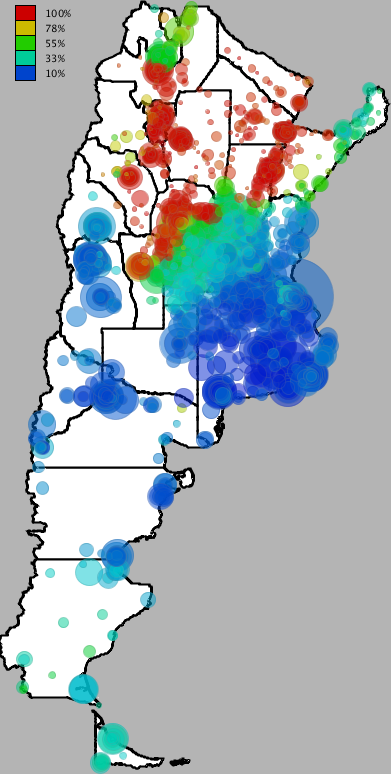
\includegraphics[width=0.90\linewidth]
  {figures/201112_hi_res_argentina_usuarios_proporcion_circulos_beta1/201112_hi_res_argentina_usuarios_proporcion_circulos_beta1}
  
(a) $\beta = 0.01$
\end{minipage}
\begin{minipage}{.495\linewidth}
\centering
  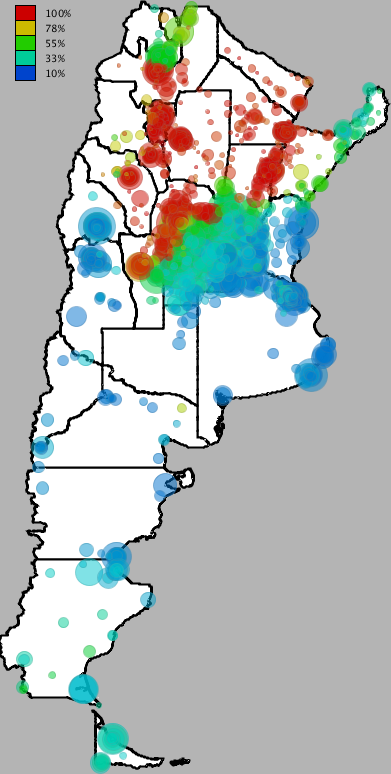
\includegraphics[width=0.90\linewidth]
  {figures/201112_hi_res_argentina_usuarios_proporcion_circulos_beta15/201112_hi_res_argentina_usuarios_proporcion_circulos_beta15}
  
(b) $\beta = 0.15$
\end{minipage}
\caption{Risk map for Argentina, filtered according to $\beta$.}
\label{fig:mapa_argentina}
\end{figure}

As a first visualization, maps were drawn using a provincial or national scale.
Advised by \textit{Mundo Sano} Foundation's experts, we then focused on areas of specific epidemic interest. 

Figure~\ref{fig:mapa_argentina} shows the risk maps for Argentina, generated with
two values for the $\beta$ filtering parameter, and fixing $m_v = 50$ inhabitants per antenna. After filtering with $\beta = 0.15$, we see that large portions of the country harbor potentially vulnerable individuals.
Namely, Figure~\ref{fig:mapa_argentina}(b) shows antennas where more that 15\% of the population has social ties with the endemic region $E_Z$.

Figure~\ref{fig:cba_sfe} shows a close-up for the Cordoba and Santa Fe provinces,
where we can see a gradient from the regions closer to the endemic zone $E_Z$ to the ones further away.


\begin{figure}[p]
\centering
  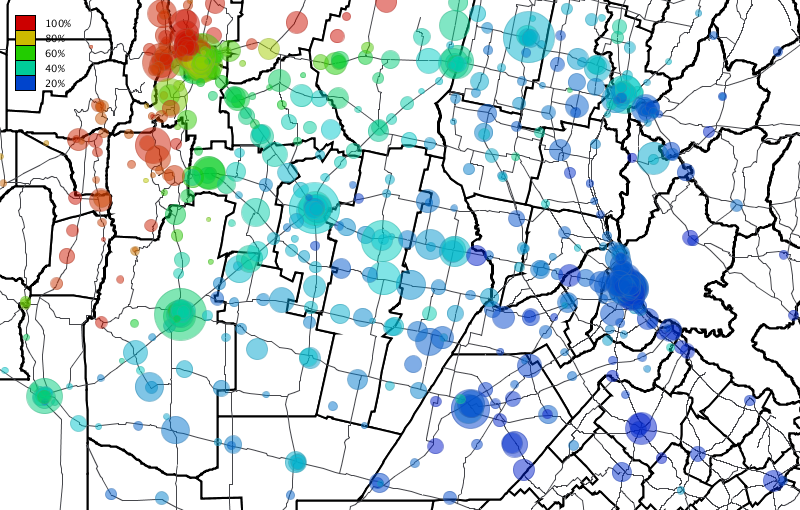
\includegraphics[width=0.95\linewidth]
  {figures/201112_hi_res_cba_sfe_usuarios_proporcion_circulos_beta15/201112_hi_res_cba_sfe_usuarios_proporcion_circulos_beta15}
\caption{Risk map for Cordoba and Santa Fe provinces, filtered according to $\beta = 0.15$.}
\label{fig:cba_sfe}
\end{figure}



\subsection{Zooming and Detection of Vulnerable Communities}
% Mapas
% Histograma de porcentaje de vulnerabilidad por antena?
% Cambios en los colores de los mapas (aclarar que el codigo de color cambia)

As a result of inspecting the maps in Figure~\ref{fig:mapa_argentina}, we decided to 
focus visualizations in areas whose results were unexpected to the epidemiological experts. 
Focused areas included the provinces of Tierra del Fuego, Chubut, Santa Cruz and Buenos Aires, with special focus on the metropolitan area of Greater Buenos Aires whose heatmap is shown in Figure~\ref{fig:amba_map}.

In some cases, antennas stood out for having a significantly higher link to the epidemic area than their adjacent antennas. Our objective here was to enhance the visualization in areas outside of Gran Chaco looking for possible host communities of migrants from the ecoregion.
High risk antennas were separately listed and manually located in political maps. This information was made available to the \textit{Mundo Sano} Foundation collaborators who used it as an aid for their campaign planning and as education for community health workers. 


\begin{figure}[p]
\centering
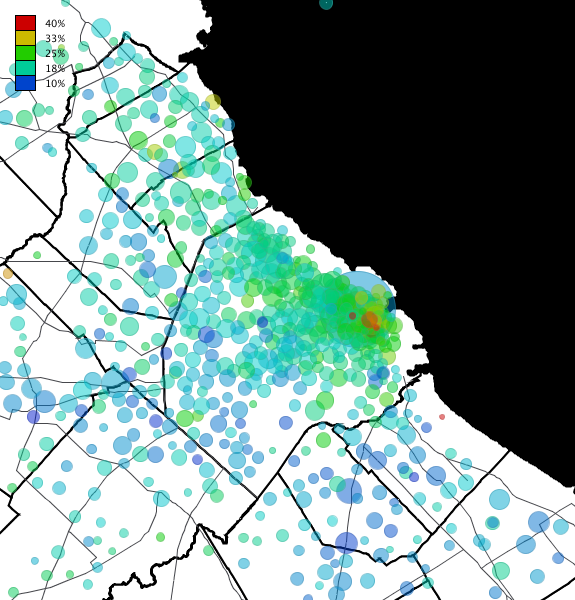
\includegraphics[width=0.75\linewidth]
{figures/201112_hi_res_amba_usuarios_proporcion_circulos_beta2/201112_hi_res_amba_usuarios_proporcion_circulos_beta2}
\caption{Risk map for the metropolitan area of Buenos Aires, filtered with $\beta = 0.02$.}
\label{fig:amba_map}
\end{figure}

\begin{figure}[h!]
\begin{center}
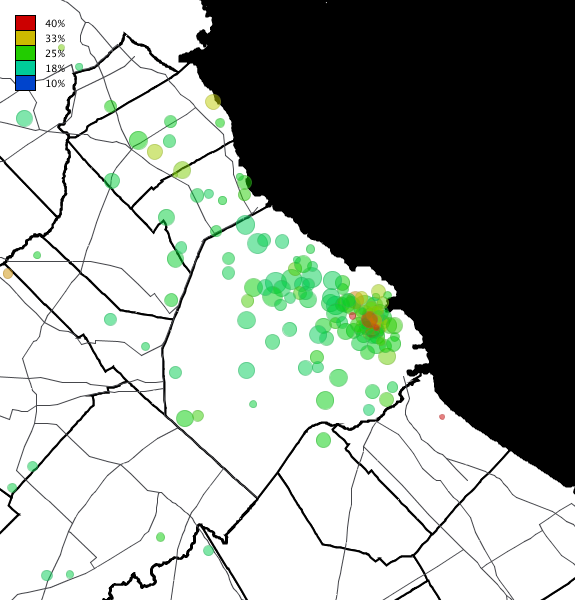
\includegraphics[width=0.35\columnwidth]{figures/201112_hi_res_amba_usuarios_proporcion_circulos_beta20/201112_hi_res_amba_usuarios_proporcion_circulos_beta20}
\caption{Replace this text with your caption%
}
\end{center}
\end{figure}

This analysis allowed us to specifically detect outlying communities in the focused regions. Some of these can be seen directly from the heatmap in Figure~\ref{fig:amba_map}, where the towns of Avellaneda, San Isidro and Parque Patricios have been pinpointed.




\subsection{Risk Maps for Mexico}

With the data provided by the CDRs and the endemic region defined in Section~\ref{endemic_zone_mexico}, heatmaps were generated for Mexico using the methods described in Section~\ref{methods}. The first generated visualizations are depicted in Figure~\ref{fig:mapas_mexico},
which includes a map of the country of Mexico, and a zoom-in on the South region of the country.
We used $m_v = 80$ inhabitants per antenna, and a high filtering value $\beta = 0.50$, which 
means that in all the antennas shown in Figure~\ref{fig:mapas_mexico},
more that 50\% of inhabitants have a social tie with the endemic region $E_Z$.
For space reasons, we don't provide here more specific visualizations and analysis of the regions of Mexico.

\begin{figure}[ht!]
\begin{minipage}{.475\linewidth}
\centering
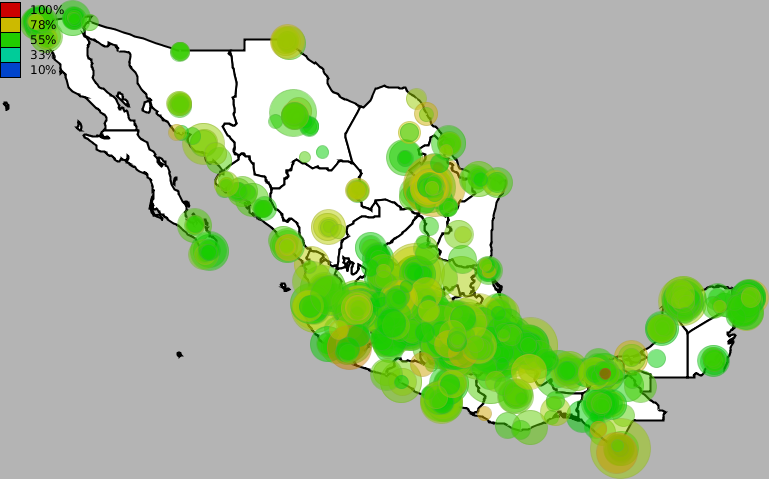
\includegraphics[width=0.95\columnwidth,height=3.2cm,keepaspectratio]
{figures/mexico_usuarios_volumen_circulos_allday_beta--50_min_volume--80_mexico_/mexico_usuarios_volumen_circulos_allday_beta--50_min_volume--80_mexico_}

(a) National map, $\beta = 0.50$
\end{minipage}
\begin{minipage}{.520\linewidth}
\centering
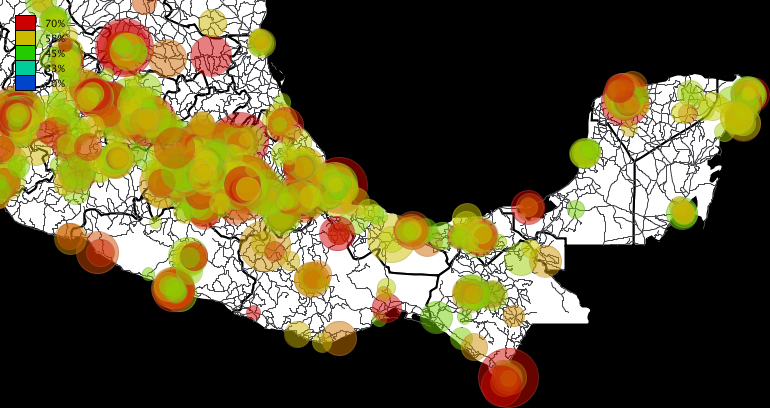
\includegraphics[width=0.95\columnwidth,height=3.2cm,keepaspectratio]
{figures/sur_usuarios_volumen_circulos_allday_beta--50_min_volume--80_mexico_/sur_usuarios_volumen_circulos_allday_beta--50_min_volume--80_mexico_}

(b) South region of Mexico, $\beta = 0.50$
\end{minipage}

\begin{minipage}{.32\linewidth}
\centering
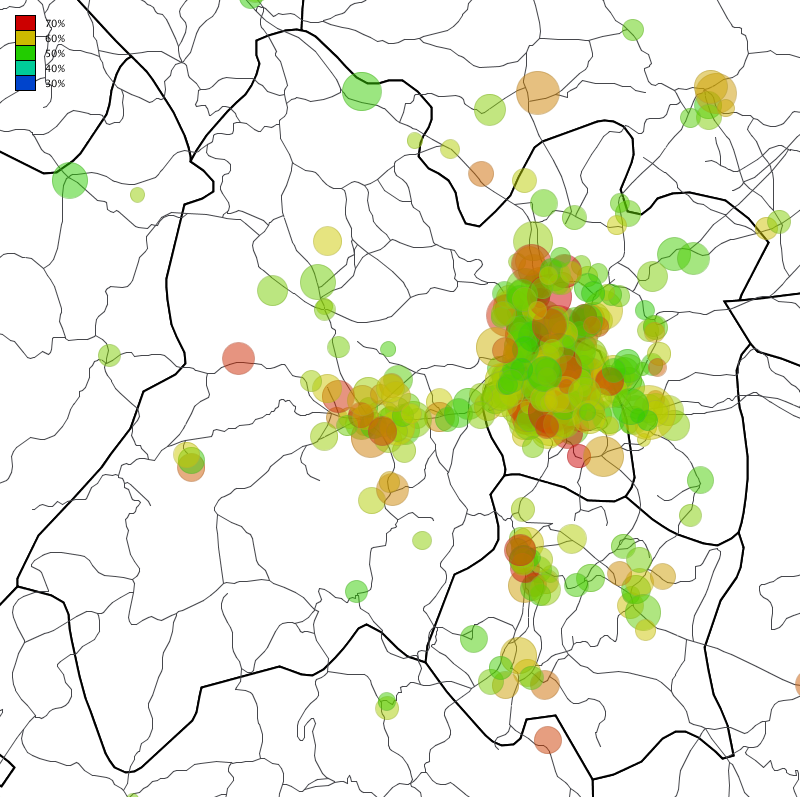
\includegraphics[width=0.90\columnwidth]
{figures/estado_mexico_usuarios_volumen_circulos_allday_beta--50_min_volume--80_mexico_/estado_mexico_usuarios_volumen_circulos_allday_beta--50_min_volume--80_mexico_}

(c) State of Mexico, $\beta = 0.50$
\end{minipage}
\caption{Risk maps for Mexico}
\label{fig:mapas_mexico}
\end{figure}






\section{Prediction of Long-term Migrations} \label{long_term}

In this section, we describe the work on the prediction of long-term mobility.
The CDR logs available for Argentina span a period of 5 months, 
whereas the Mexican dataset includes 24 months, from January 2014 to December 2015, making it more suitable for this study.

We divide the available data into two distinct periods:
$T_0$, from January 2014 to July 2015, considered as the ``past" in our experiment;
and $T_1$, from August 2015 to December 2015, considered as the ``present".
Knowing which users live in the endemic region $E_Z$ and how they communicate
during period $T_1$,
we want to infer whether they lived in $E_Z$ in the past (period $T_0$).
Our target variable $Y$ is thus defined in the following way for every user $u$,
where $H_u$ is the user's home antenna: 
\[
    %\begin{equation}
    Y_u =
      \begin{cases}
        &1 \ \mbox{if} \ H_u \in E_Z \mbox{ during } T_0 \\
        &0 \ \mbox{in other cases}.
      \end{cases}
    %\end{equation}
    \]
With this target variable, we tackle the prediction as a supervised classification problem.


\subsection{Training Set}

As explained, the training data belongs to period $T_1$, from August 2015 to December 2015;
whereas the ground truth that we use to validate the predictions belongs to $T_0$, from January 2014 to August 2015.
After preprocessing and cleaning the dataset, we obtained 
a training set with 1.6 million users.

Table~\ref{tab:distribution_by_state} shows the percentage of antennas, the percentage of the population (according to INEGI census 2014), and
the percentage of telco users per state, for the top 10 states.
% (wikipedia \url{https://en.wikipedia.org/wiki/Ranked_list_of_Mexican_states})


\begin{table}[ht]
\caption{Distribution of antennas, population and telco users by state.}
\label{tab:distribution_by_state}
\centering
\begin{tabular}{l r r r}
\toprule
State				& Number of antennas & Population 	& Telco users \\
\midrule
Distrito Federal    & 28.2\% 	& 8.5\%		& 20.1\%  \\
Mexico              & 21.2\%		&  13.9\% 	& 23.8\%  \\
Jalisco             & 10.7\% 	& 6.4\%		& 8.3\%   \\
Nuevo Leon          & 9.6\%	& 4.9\%		& 2.9\% \\
Guanajuato          & 6.1\%	& 4.8\%		& 5.9\% \\
Puebla              & 5.8\%	& 5.3\%		& 4.3\% \\
Veracruz            & 5.4\% 	& 6.8\%		& 4.2\% \\
Baja California     & 4.3\%	& 2.8\%		& 1.1\% \\
Yucatan             & 4.1\%	& 1.7\%		& 2.9\% \\
Sinaloa             & 4.1\%	& 2.5\%		& 0.4\% \\
\bottomrule
\end{tabular}
\end{table}

The raw data logs contain between 11 million and 30 million calls per day and the volume of calls increases over the months, where most recent months have higher rates.

In this analysis we considered only postpaid users, i.e., users which have a monthly  plan rate. This filtering was done because prepaid users have a higher churn rate, thus meaning that phone lines are not necessarily associated with one single person during the two years of analysis, making them less suitable for the purpose of this study.

% (i.e. cellphone lines might ``jump" suddenly from one region to another).

% Data was manipulated to build a ??


\subsection{Model Features}

The quality of the classification relies on the ability to characterize the users and their communication patterns. % as differentiating as possible. 
In general, the features constructed reflect calling and mobility patterns,
segmented by different time periods during the week, and tagging whether the actions or subjects are `endemic'. 
The training data runs from August 2015 to December 2015 (period $T_1$) and all CDRs are processed to extract features by user and by link. 

Each week is divided into 3 time periods: (i) the period \textit{weekday} is from Monday to Friday, on working hours (from 8hs to 20hs); (ii) \textit{weeknight} is from Monday to Friday, between 20hs and 8hs of the following day;
and (iii) \textit{weekend} is Saturday and Sunday.

The model consists of the following features, which can be classified in 4 categories:
% The data is aggregated by user and by link.0


\subsubsection{Used and home antennas.}\label{homeantenna}

For each user $u \in \calN_C$, we register the top ten most used antennas, during each month of the training period,
together with the number of calls made through each antenna. We tag all users having their home antenna in the epidemic region as \textit{EPIDEMIC}. 
%Which 10 antennas does a user use most during each month of the training month interval? 
%
%How many calls have been made through each antenna? 
%
%Sort antennas with 0 being the most used and 10 the least used. Fill with nulls when less than 10 antennas were used.
We also register the most used antennas considering only calls made during the \textit{weeknight} period, as defined above. % that is from Monday to Friday excluding the working hours (from 8hs to 20hs)\label{WEEKNIGHT}.
% Log counts as well.

A user's home antenna is defined by the most used antenna during the \textit{weeknight} period in all of $T_0$.
%5 months. 
From this, users were tagged as `endemic' if their home antenna is in the endemic zone $E_Z$ and `exposed' if any of the ten antennas logged is in the risk area.


\subsubsection{Mobility diameter.}

The user's logged antennas define a convex hull in space and the radius of the hull is taken to be as the mobility diameter. This length is representative of the area of influence of that individual, a feature expected to be correlated with long-term migrations.

We register the mobility diameter of each user, as the diameter of the convex hull defined by his top 10 used antennas. Again, we generate two values, considering (i) all antennas and (ii) only the antennas used during the \textit{weeknight}.



\subsubsection{Graph data and communications.}




We look at the social graph $\calG_C$ built from the CDRs, and the communications between nodes in $\calN_C$.

	For each edge $\left< n_i, n_j \right> \in \calE_C$, we dive into each of their interactions, segmenting call data with different criteria. For %\textbf{each} 
	each month and each pair of users $\left< i,j \right>$, we gather the tuple $\left< time_{ij}, calls_{ij}, dir, period \right>$ where $time$ is the sum of all calls (in seconds), $calls$ is the number of calls exchanged, $dir$ is a boolean variable indicating whether the calls were incoming or outgoing (from user $i$'s point of view) and $period$ corresponds to a segmentation of the week into the periods \textit{weekday}, \textit{weeknight}, and \textit{weekend}.


In this sense, two users $u_i, u_j \in \calN_C, u_i \neq uj$ are \textbf{neighbors} in the social graph if $time_{ij} > 0$.

%\begin{description}
%    \item [Neighbors.] From the social graph built from the CDRs we extracted the total count of neighbors in the communication graph and the total count of epidemic neighbors. 
%    \item [Calls.] For each month, the total time and count of monthly calls made during is aggregated per user. This information is also segmented according to the hour of the day that the calls were made and whether they were made during the weekends. Special care was taken with calls placed to and from vulnerable users and aggregated accordingly.
%\end{description}

%if we find that user $j$ is epidemic. This may be translated as the edge is vulnerable if one of both users is epidemic.

Since the samples in our dataset are users, we have to aggregate all these variables, by grouping interactions at the user level. The combination of different variables amounts to a total of 130 features per user.
 
To illustrate the point, we show a small example of how two calling features could look like. Groupings and filters are applied only on the user's calls:

\begin{table}[ht]
	\caption{Graph Data Features Example}
	\label{tab:data_example}
	\centering
	\begin{tabular} {|p{1.5cm}|p{1.5cm}|p{2cm}|p{1.5cm}|p{2cm}|p{1.5cm}|p{1cm}}
		%{l r r r r r r }
		\toprule
		Feature name & Call/Time & Time Period & Direction & Endemicity & Month\\
		\midrule
		Calls WeekEnd InVul08     & Count of calls & Placed on WeekEnds & Incoming calls & Edges with endemic neighbours only & August\\
		\midrule
		Time WeekNight Out12 & Sum of duration in seconds & During weekdays and on out-of-office hours & Outgoing  & No endemic filtering  & December \\
		
		\bottomrule
	\end{tabular}
\end{table}


 TimeWeekNight_OUT_12

 CallsWeekEnd_IN_12

Finally we aggregate all these variables at the user level, summing over all columns and grouping by user. 
 (either $j$ or $i$) by summing across all of the different ??components?? (group by user, sum over all columns) .

 We also label each edge $\left< n_i, n_j \right> \in \calE_C$ if one or both users is endemic.
We also count each user's amount of neighbors in the communication graph and the total count of endemic neighbors, labeling each user $i$ as \textit{vulnerable} whenever he has any edge with another user $j$ who lives in the endemic region $E_Z$. 

%% el vulnerable NO es el edge, sino que es el usuario . 
%La idea es, parate en el nodo i, hace algun filtro - o ninguno - de weeknight, in/out, weekend, mes, etc. y ahora decime
%% if $\exists j$ such that edge $ij$ existe en el grafo de llamados (con el filtro que hayamos usado en ese momento puesto).
%%

%Additionally, for each user, we extract the total 


\subsubsection{Validation data.} % {Ground Truth.}

We perform an analysis similar to the home antenna detection previously described, 
but considering the time period $T_0$ (from January 2014 to July 2015),
in order to determine the home antenna of users during $T_0$.

The number of people who maintain their home antenna between $T_0$ and $T_1$ is 1,012,416;
whereas 580,425 users had a change in their home antenna.
In terms of endemic condition, we observed that 1,551,560 users maintained their endemic condition
between $T_0$ and $T_1$, whereas 41,281 had a change.

%We consider two versions, the most used antenna (without filtering), and the most used antenna during the \textit{week night}.


%Dato de color:
%Num de personas que mantiene su home antenna en los dos periodos: 1012416 cambio: 580425
%
%Num de personas que mantiene su $antenna_id_0$ (most used antenna, sin filtro de nada) en los dos periodos: 1052644 cambio: 540197
%
%Num de personas que mantiene su condicion de epidemicidad en los dos periodos: 1551560 cambio: 41281
%
%Refinando la epidemicidad:

% Confusion matrix
Table~\ref{tab:changes} 
shows the matrix of changes $C$, such that $C_{i, j}$ is the number of users that were in group $i$ during period $T_0$ (the past) and moved to group $j$ during the training period $T_1$. As an example, lower left means was endemic, is now not endemic. 

\begin{table}[ht]
\caption{Matrix of endemicity change}
\label{tab:changes}
\centering
\begin{tabular}{l r r }
\toprule
				& Not endemic in $T_1$ & Endemic in $T_1$ \\
\midrule
Not endemic in $T_0$ & 1140360 & 18330  \\
Endemic in $T_0$     & 22951   & 411200 \\
\bottomrule
\end{tabular}
\end{table}

In relative numbers, this shows that only 2.59\% of users had a change in their endemic condition over time. A similar count shows that 66.0\% of users have not changed their home antenna from $T_0$ to $T_1$.


% \subsection{Supervised Algorithms}
\subsection{Supervised Classification}


In this first iteration, we used the most common techniques found in the literature for this task:
Support Vector Machines, Random Forest, Logistic Regression, and Multinomial Naive Bayes.

All algorithms were run on a 16-core Linux machine with 72GB of RAM.  Processing and learning scripts were run on Python. %\footnote{Python Software Foundation. Python Language Reference, version 3.5. Available at http://www.python.org}. 
Along the project, a variety of external packages were used for different purposes. For the classification routines, we used Scikit-learn~\cite{sklearn} and Graphlab~\cite{graphlab}.
The data was split into 70\% for training and 30\% for testing.


%\cite{Python}
%\cite{sklearn}
%\cite{graphlab}

Random forests, Gradient Boosting, Logistic Regression and Support Vector Machines are standard for this kind of jobs. For the purpose of fast benchmarking, Multinomial Naive Bayes is also tested since it is a very fast non-parametric method. 

Where possible, feature importance methods will be used to quantify the contribution of the feature or the interaction of features to the mobility of the users.


% Algorithms: SVM, Random Forest and Logistic Regression, Multinomial Naive Bayes


\subsubsection{Multinomial Bayes.}
 
 The Multinomial Bayes classifier has a linear time complexity, and thus serves as a fast benchmark that we used to establish a baseline classification performance. However, one shortcoming of this method is that it only allows for non-negative numerical features. This results in a reduced training and testing set.
  
 The classifier has two hyperparameters: $\alpha$, an additive smoothing parameter for which we defined values of $[0,{10^{-2}},{10^{-1}},1]$; and the \textit{fit prior} parameter which determines whether or not class prior probabilities are learned from the training set. 
 
 This setup gave 8 possible models and 24 fits on the 3-fold cross validated model training set where, on average, learning took 5s for one million samples. The F1-weighted metric was chosen to evaluate the best performing estimator.
The best and worst scores achieved were 0.940 and 0.918 respectively. 
 % which gave a score of 0.9409381515 noting that the worst estimator had a score of 0.918.

A full classification report on the out of sample data is shown below, where values are detailed for each target class:
\begin{table}[ht]
	% \caption{Matrix of changes.}
	\label{tab:classification_report}
	\centering
	\begin{tabular}{ l r r r r }
		\toprule
		{ } & precision score & recall  & f1-score & support \\
		\midrule
		0 		  & 0.96 & 0.96  & 0.96 & 323278  \\
		1		  & 0.89 &  0.90 &  0.90 & 411200 \\
		avg/total & 0.94 &  0.94 &  0.94 & 445464 \\
		\bottomrule
	\end{tabular}
\end{table}

%  precision    recall  f1-score   support 
%  0       0.96      0.96      0.96    323278
%  1       0.89      0.90      0.90    122186
 % avg / total       0.94      0.94      0.94    445464  

\subsubsection{SVM and Logistic Regression.}

Support Vector Machines (SVM) and Logistic Regression are two algorithms for classification which are standard in the Machine Learning literature and performed better than Multinomial Bayes in this case. 
At the same time, they are more complex and have higher time complexity, taking more computational resources to optimize.

Only the standard hyperparameters for these two models were tuned: $L2$-penalty regularization for Logistic Regression and kernel bandwidth for the Gaussian Kernel SVM.
Both learning routines were executed in parallel and in each iteration 5\% of the training set was sampled for cross validation. The best classifier was selected based on accuracy scores from this set.

% L-BFGS is the optimization routine.  limited memory Broyden–Fletcher–Goldfarb–Shanno 
%(reference the limited memory Broyden–Fletcher–Goldfarb–Shanno (BFGS) algorithm \url{https://en.wikipedia.org/wiki/Limited-memory_BFGS} )
%% es un algoritmo de optimizacion numerica para computar minimos de funciones


% With a running time of 80s, 10 steps are generally needed to achieve a 0.977 validation accuracy score on 
The best model was a Logistic Regression Classifier with an $L2$-penalty value of 0.01. 
% Table~\ref{tab:results} 
The following table
shows the scores obtained by the selected model on the out-of-sample set.

\begin{center}
\begin{tabular}{ l l }
\toprule
Score & Value \\
\midrule
F1 score  & 0.964537   \\
Accuracy  & 0.980670   \\
AUC       & 0.991593   \\
Precision & 0.970838   \\
Recall    & 0.958316   \\
\bottomrule
\end{tabular}
\end{center}


\begin{table}[ht]
\caption{Resulting scores.}
\label{tab:results}
\centering
\begin{tabular}{ l l }
\toprule
Score & Value \\
\midrule
F1 score  & 0.964537   \\
Accuracy  & 0.980670   \\
AUC       & 0.991593   \\
Precision & 0.970838   \\
Recall    & 0.958316   \\
\bottomrule
\end{tabular}
\end{table}

High values across all scoring measures are achieved. % with the best estimator, with the lowest metric starting at a value of 0.958. 
These results can be explained by the fact that 
%Scores results become less surprising when looking closer at the dataset. 
communication and mobility patterns are in essence highly correlated across time periods. 
In this case, correlation between the target variable $Y$ and the models' features are expected:
% The table below shows the top 7 target-correlated features. 
a user being endemic in $T_1$ is very correlated to being endemic in $T_0$, and the same holds with a user's interaction with vulnerable neighbors during $T_1$.

% \hfill
\begin{table}
% \parbox{0.45\linewidth}{
\caption{Correlations.}
\label{tab:results}
\centering
\begin{tabular}{l l }
\toprule
Feature & Correlation \\
\midrule
Endemic in $T_1$               & 0.943801 \\
Vuln. contact outgoing 08/2015    & 0.730294 \\ %%outgoing significa outgoing calls
Vuln. contact incoming 08/2015     & 0.732498 \\
Vuln. contact outgoing 09/2015    & 0.714448 \\
Vuln. contact incoming 09/2015     & 0.715566 \\ 
Vuln. contact outgoing 10/2015    & 0.694106 \\
Vuln. contact incoming 10/2015     & 0.694265 \\
%VULNERABLE\_OUT\_11    & 0.688250 \\
%VULNERABLE\_IN\_11     & 0.688407 \\
\bottomrule
\end{tabular}
\end{table}


%
%Si del test\_set ahora me quedo con lo users que Y\_target ==1 == EPIDEMIC\_gt pero que hoy en dia son epidemic ==0 (se mudaron). Los scores bajan mucho:
%
%+--------------+-----------------+-------+
%| target\_label | predicted\_label | count |
%+--------------+-----------------+-------+
%|      1       |        1        |  1944 |
%|      1       |        0        |  3525 |
%+--------------+-----------------+-------+
%'f1\_score': 0.5244840145690004, ''accuracy': 0.3554580,, 'precision': 1.0, 'recall': 0.35545803, 


\section{Conclusions and Future Work}

\subsection{Summary of Results}

The heatmaps shown in Section~\ref{results} expose a ``temperature'' descent from the core regions outwards. The heat is concentrated in the ecoregion and gradually descends as we move further away. This expected behavior could be explained by the fact that calls are in general of a local nature and limited to 3 or 4 main antennas used per user. 

A more surprising fact is the finding of communities atypical to their neighboring region. They stand out for their strong communication ties with the studied region, showing significantly higher links of vulnerable communication. The detection of these antennas through the visualizations is of great value to health campaign managers. Tools that target specific areas help to prioritize resources and calls to action more effectively.

In Section~\ref{long_term}, we tackled the problem of predicting long-term migrations. In particular, we showed that it is possible to use the mobile phone records of users during a bounded period (of 5 months) in order to predict whether they have lived in the endemic zone $E_Z$ in a previous time frame (of 19 months).
The very good results obtained demonstrate that CDRs are particularly well suited for this task.
 
To conclude, the results presented in this work show that it is possible to explore CDRs as a mean to tag human mobility. Combining social and geolocated information, the data at hand has been given an innovative use, different from its original billing purpose.

Epidemic counter-measures nowadays include setting national surveillance systems, vector-centered policy interventions and individual screenings of people. These measures require costly infrastructures to set up and be run. However, systems built on top of existing mobile networks would demand lower costs, taking advantage of the already available infrastructure. The potential value these results could add to health research is hereby exposed.
Finally, the results stand as a proof of concept which can be extended to other countries or to diseases with similar characteristics.



\subsection{Lines for Future Work}

The mobility and social information extracted from CDRs analysis has been shown to be of practical use for Chagas disease research. Helping to make data driven decisions which in turn is key to support epidemiological policy interventions in the region. For the purpose of continuing this line of work, the following is a list of possible extensions being considered:

\begin{description}
    \item [Results validation.] Compare against actual serology or disease prevalence surveys. Data collected from fieldwork could be fed to the algorithm in order to supervise the learning. 
    
    \item [Differentiating rural antennas from urban ones.] This is important as rural areas have conditions which are more vulnerable to the disease expansion. \textit{Trypanosoma cruzi} transmission is favored by rural housing materials and domestic animals contribute to complete the parasite's lifecycle. Antennas could be automatically tagged as rural by analyzing the differences between the spatial distribution of the antennas in each area. A similar goal could be to identify precarious settlements within urban areas, with the help of census data sources.

    \item [Seasonal migration analysis.] Experts from the \textit{Mundo Sano} Foundation underlined that many seasonal migrations occur in the \textit{Gran Chaco} region. 
    Workers might leave the endemic area for several months possibly introducing the parasite to foreign populations.
      The analysis of these movements can give information on which communities have a high influx of people from the endemic zone.
    %\item Add more regions to the analysis.

    \item [Search for epidemiological data at a finer grain.] For instance, specific historical infection cases. Splitting the endemic region according to the infection rate in different areas, or considering particular infections.
    \item Feature exploration to search for correlations with being infected.
    %\item (FALTA RESCRIBIR) Apply best fit model to Argentinian dataset. Provide that info to a Chagas risk model. Assuming that a high influx of individuals from epidemic regions is correlated with a higher risk in that area the algorithm could highlight these points. % revisar
\end{description}
